\section*{Задача 4.1}
\subsection*{Постановка задачи}
В таблице приведены данные о численности населения некоторых
крупнейших стран мира по годам с 1950-2000 г.г. Заполнить последние два столбца
таблицы (взять сведения из интернета). На основе этих данных для конкретного варианта
построить наилучший многочлен по МНК. Найти численность населения страны в 2019
году и сравнить полученное значение с актуальным значением (взять из интернета).
Решить ту же задачу на основе интерполяционного многочлена. То есть построить
интерполяционный многочлен по значениям с 1950-2020 г.г. Вычислить значение для
2019 года и сравнить с актуальными данными.

\begin{tabular}{| c | c | c | c | c | c | c | c | c | c |}
	\hline
	N & Страна & 1950 & 1960 & 1970 & 1980 & 1990 & 2000 & 2010 & 2020 \\ \hline
	4.1.33 & Чехия & 8.9 & 9.6 & 9.9 & 10.3 & 10.4 & 10.3 & 10.5 & 10.7 \\ \hline
\end{tabular}

\subsection*{Теоретический материал}

Требуется найти многочлен $P_m$ заданной степени $m, (m < n)$ такой, чтобы величина
среднеквадратичного отклонения (СКО)
\[
	\sigma(P_m, f) = \sqrt{\dfrac{1}{n + 1}\sum\limits_{i=0}^n(P_m(x_i) - f_i)^2}
\]
была минимальной. Для нахождения этого минимума будем использовать условие экстремума функции нескольких переменных:
\[
	\dfrac{\partial \rho}{\partial a_k} = 0, k = 0,1 \dots m
\]

Таким образом задача о нахождении многочлена  степени $m$ сводится к поиску решения следующей симметричной системы:

\[
	\begin{cases}
		s_0a_0 + s_1a_1 + s_2a_2 + \dots + s_ma_m = b_0 \\
		s_1a_0 + s_2a_1 + s_3a_2 + \dots + s_{m+1}a_m = b_1 \\
		\dots \\
		s_ma_0 + s_{m+1}a_1 + s_{m+2}a_2 + \dots + s_{2m}a_m = b_m \\
	\end{cases}
\]

Где $
\begin{array}{c c}
	s_k = \sum\limits_{i=0}^nx_i^k & b_k = \sum\limits_{i=0}^n f_ix_i^k
\end{array}
$

Остается опытным путем определить, какую степень многочлена $m$ необходимо взять, чтобы получить наилучшее приближение, так как с ростом $m$ среднеквадратичное отклонение сначала убывает, а затем начинает возрастать, причем при больших $m$ нормальная система наименьших квадратов становится плохо обусловленной, а при $m = n$ многочлен совпадает с интерполяционным многочленом.

Решим ту же задачу с помощью интерполяционного многочлена, записанного в форме Лагранжа:

\[
	L_n(x) = \sum\limits_{i=0}^n f_i \prod\limits_{k=0}^n\dfrac{(x - x_k)}{(x_i - x_k)}, (i \ne k)
\]

\subsection*{Решение}

Прежде чем разрабатывать алгоритм решения данной задачи, сформулируем несколько требований к основной подпрограмме:

\begin{itemize}
	\item На вход подпрограмме подается 2 массива - массив аргументов и массив значений
	\item На выход подпрограмма возвращает функцию, реализующую искомый многочлен
	\item Для решения задачи методом наименьших квадратов также необходима функция, вычисляющая среднеквадратичное отклонение.
\end{itemize}

Теперь опишем алгоритм решения задачи по методу наименьших квадратов:

\begin{enumerate}
	\item Опишем вспомогательные функции, позволяющие вычислить коэффициенты $s_k$ и $b_k$ нормальной системы наименьших квадратов.
	\item Сформируем матрицу системы и решим ее с помощью встроенного метода библиотеки NumPy  np.linalg.solve()
	\item В качестве конечного результата сформируем функцию, реализующую искомый многочлен.
	\item В конце необходимо "подобрать" степень многочлена, сравнивая среднеквадратичные отклонения для различных $m$.
\end{enumerate}

Для построения интерполяционного многочлена в форме Лагранжа используем прямую формулу, то есть по определению.

\subsection*{Анализ результатов}

Анализ среднеквадратичных отклонений показал, что наименьшее свое значение оно показывает при степени многочлена $m = 4$. Ниже представлены графики обоих многочленов.

\noindent
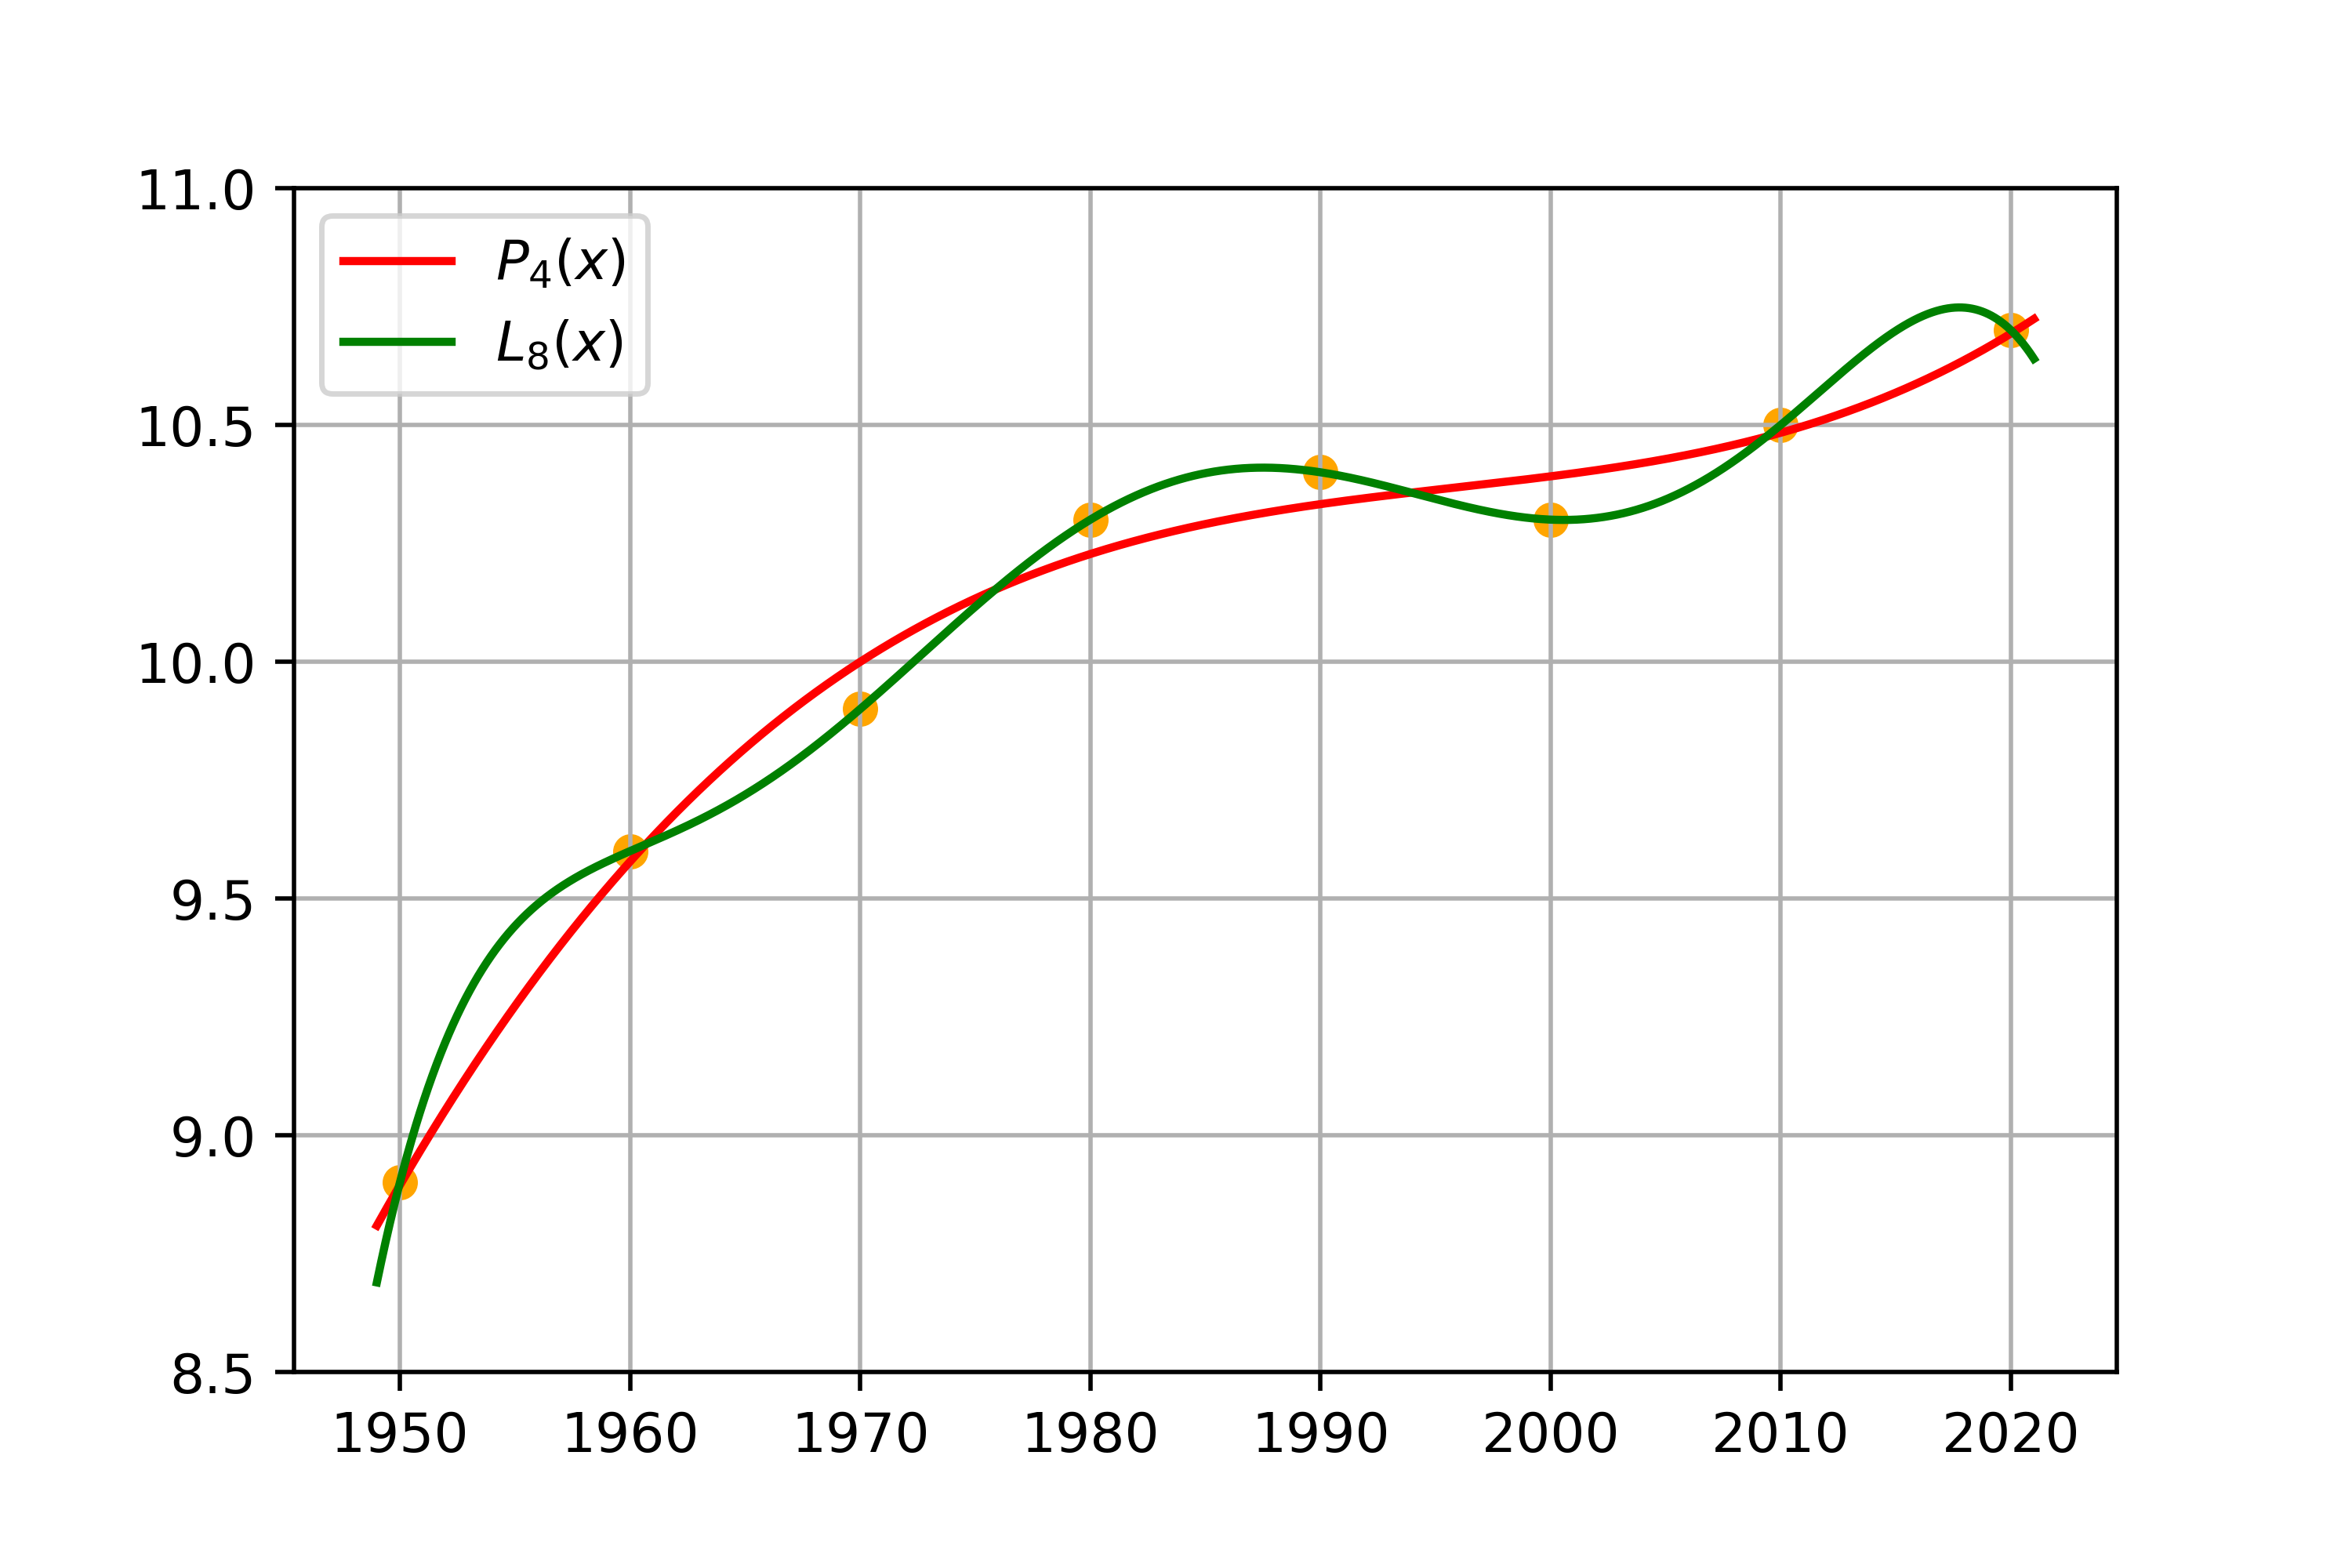
\includegraphics{images/plot_4.1.png}

Вычислив значение численности населения Чехии в 2019 году, и сравнив их с реальным значением получили следующие реузльтаты:

\begin{tabular}{l}
	Метод наименьших квадратов: 10.664 \\
	Интерполяционный многочлен: 10.734 \\
	Реальное значение: 10.669 \\
\end{tabular}

Метод наименьших квадратов дал более точное значение в связи с тем, что такие данные, как численность населения заданы с некоторой погрешностью, из-за чего полином, полученый с помощью МНК, дает более точное представление о динамике численности населения.
\newpage
\subsection*{Код программы}

\begin{lstlisting}
import numpy as np
import matplotlib.pyplot as plt

x = [1950, 1960, 1970, 1980, 1990, 2000, 2010, 2020]
y = [8.9, 9.6, 9.9, 10.3, 10.4, 10.3, 10.5, 10.7]

def Least_Squares(x: list, y: list, m: int):
    s = lambda k: sum([elem**k for elem in x])
    b = lambda k: sum([y[i]*x[i]**k for i in range(len(x))])
    NormalSystem = np.zeros((m+1, m+1))
    for i in range(m+1):
        for j in range(i, m+1):
            temp_coef = s(i + j)
            NormalSystem[i, j] = temp_coef
            NormalSystem[j, i] = temp_coef
    d = np.array([b(i) for i in range(m+1)])
    a = np.linalg.solve(NormalSystem, d)
    return a

def Average_Square_Deviation(Polynom, x, y):
    return (1.0/(len(x)) * sum([(Polynom(x[i]) - y[i])**2 for i in range(len(x))]))**0.5

devs = []
for m in range(1, 6):
    a = Least_Squares(x, y, m)
    Polynom = lambda x: sum([a[i]*x**i for i in range(m+1)])
    devs.append(Average_Square_Deviation(Polynom, x, y))
print(devs)#min(dev) = 0.060136. Polynom degree - 4

a = Least_Squares(x, y, 4)
Polynom = lambda x: sum([a[i]*x**i for i in range(5)])

def Lagrange_Polynom(arg):
    res = 0
    for i in range(len(x)):
        tmp = 1
        for k in range(len(x)):
            if i != k:
                tmp *= (arg - x[k]) * 1.0/(x[i] - x[k])
        res += y[i]*tmp
    return res

print("Least Squares method:", Polynom(2019))
print("Lagrange Polynom:", Lagrange_Polynom(2019))
print("Real value:", 10.669)
\end{lstlisting}